\chapter{Introduction}
Recommendation systems were introduced in the 1990s; since their introduction, recommendation systems (RS) have continually evolved and are now adopted by most modern technology companies. These information filtering systems use either matrix factorization or collaborative filtering to predict which content elements will be most suitable for each user. These content-based systems require large amounts of user and recommendation data~\cite{ref1}. Generally, the more data an RS uses, the better its recommendation performance. To make practical suggestions, the RS needs as much information as possible from the user. They collect personal data, including actions, context, domain details, purchase history, responses to recommendations, social media profiles, and more. To improve accuracy, several recommender systems combine data from many sources. Altogether, this valid user data is kept in a single location within each company's database to support various recommendation services~\cite{ref2}.

\section{Motivation for the Study}
Since an RS can only use the data, it has available to make predictions, the more and better-quality user information it has, the more accurate those predictions will be. Many advertising firms and advertisers have used various RS tools and utilities, along with third-party cookies, to gather this data. To deliver personalized ads based on user profiles, third-party cookies track and store users' online activities. These systems can be invasive and breach privacy by recording everything users do online, including their destinations, clicks, visited pages, age, gender, and more~\cite{ref2}. The information of 145 million eBay customers, such as their names, addresses, birthdays, and passwords, was leaked after hackers attacked the company in May 2015~\cite{ref91}. Facebook revealed the private data of tens of millions of users in March 2018~\cite{ref92}. Large-scale breaches of personal data happen often at internet companies due to similar incidents. The increasing volume of data provides chances to discover valued insights and develop smart applications. However, gathering large quantities of user data raises concerns about privacy and security. Advances in technology make protecting customer data even more important. Consumers expect privacy safeguards in every transaction; many everyday activities, whether through online banking or mobile apps, put personal data at risk. Governments around the world were initially slow to establish laws and regulations. This is to shield sensitive information from cybercrime, identity theft, and other privacy breaches.

Nonetheless, the landscape is changing as data protection laws are being enacted worldwide. Multiple factors drive the rise of these rules. This includes the spread of large quantities of data, which requires better data security and privacy measures to protect users from malicious threats. The ``Digital Personal Data Protection Act'' of 2023 in India~\cite{ref3}. The ``California Consumer Privacy Act'' (CCPA)~\cite{ref4}, the ``Colorado Privacy Act'' (CPA)~\cite{ref5}, and the European Union's ``General Data Protection Regulation'' (GDPR)~\cite{ref6}, are all essential laws that protect personal data and keep it private in different places~\cite{ref7}.

While developing the machine learning model, more sensitive data were used. Membership inference and model inversion attacks are two examples of many privacy leakage vulnerabilities in machine learning models. Several privacy concerns compromise data security and make owners less willing to share their information with machine learning (ML) systems. Without sufficient training data, ML systems will have minimal applications. Data owners need to pre-assess potential datasets and implement appropriate privacy controls; therefore, analyzing privacy risk mitigation strategies is crucial. On the other hand, data owners still lack access to comprehensive privacy risk assessments. The public's understanding of the significance of safeguarding individual data and preventing its collection by online services has increased~\cite{ref8}. Federated learning is a better choice than traditional machine learning because it is decentralized, which makes it safer and better for privacy.

Personalized recommendations are essential for enhancing user experience across many fields. However, collecting large quantities of user data raises concerns pertaining to data privacy and security. As technology advances, protecting client data has become more critical. Integrating Federated learning with recommendation systems helps address privacy and security problems, but most existing federated recommendation systems are built on simulated frameworks and lack real-time capabilities.

\section{Present Status}
Data is collected using the traditional big data approach to create large data storage systems. Machine learning (ML) is used to address specific issues within these large data warehouses. The resulting model, when deployed, is highly generalizable with large training data. Continuous data collection, however, consumes a lot of bandwidth for transmission. Privacy-related apps may simply prevent any communication of data, which will not allow model development. It is computationally expensive to train large ML models on large data repositories, and the traditional centralized training process is limited by the performance of one machine. Delays between the incremental updates to the model are high because of slow training methods, which makes it less flexible to changing data patterns. Conversely, in an FL system, training is performed at the data sites. The trained models of all the clients are sent to the central server. These models are aggregated using aggregation methods to create an aggregated model. The new model parameters are then distributed to the data sites to train them further. Because data is never relocated, training is done locally at the data site, which supports data privacy. Asynchronous learning is an effective and scalable distributed learning approach because training can run on different nodes. In FL, the nodes and the server merely communicate model weights, which significantly minimizes communication overhead. Superior aggregation algorithms can ensure training performance and enhance efficiency in traditional ML contexts even in small-scale situations.

\subsection{Federated Learning}
The emergence of Federated Learning connects far-flung data sources and emphasizes information safety and privacy, which promotes the formation of reliable, robust machine learning systems. Federated Learning (FL) was first announced in 2016 by McMahan et al. as a tool to enhance the performance of on-device speech recognition and text input in smartphones. The Google team created a system that used users' mobile devices to gather local interaction data and continuously improve the local-language forecasting system. The Federated Averaging algorithm combines the results of SGD run on the client's device with those from a central server, enhancing the global model. Studies on FL are conducted in diverse areas focused on protecting privacy and data security~\cite{ref9}. FL is a distributed machine learning approach in which tasks traditionally managed by a central server are distributed. This system facilitates cooperation among clients, rather than requiring them to control the entire process in a conventional DML arrangement. Another prominent benefit of it is the extra privacy and security. Federated learning architecture is based on smart equipment such as cell phones and sensors, which accumulate and process the data on the local station and, in the process, store sensitive material on the device of the individual at all times. Rather, the client builds a sub-model in his/her local environment and transmits encrypted changes to the server where they are incorporated into the global model.

The strong privacy protections offered by federated learning make it an appealing option in environments where data breaches and theft are common and serious risks~\cite{ref10}. The step-by-step process is tabulated below.

\setlength{\tabcolsep}{3pt}
\begin{longtable}{|p{0.9cm}|p{10.4cm}|p{4.0cm}|}
\caption{Federated Learning Step-wise Process}\label{tab:ch1_t1}\\
\hline
\textbf{Step No.} & \textbf{Action to be taken} & \textbf{Graphical Presentation} \\
\hline
\endfirsthead
\hline
\textbf{Step No.} & \textbf{Action to be taken} & \textbf{Graphical Presentation} \\
\hline
\endhead
1 & Select a pre-trained or an untrained model on the server. & 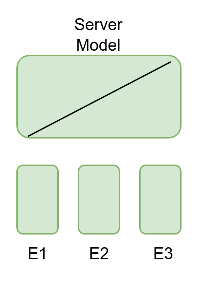
\includegraphics[height=2.7cm,keepaspectratio]{figures/fl_step_1.png} \\
\hline
2 & Distribute the initial model to the clients (devices or local servers). & 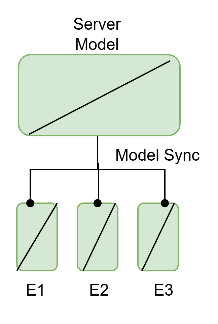
\includegraphics[height=2.7cm,keepaspectratio]{figures/fl_step_2.png} \\
\hline
3 & Every customer keeps training it locally with their own data. & 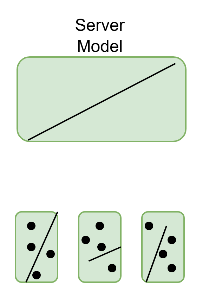
\includegraphics[height=2.7cm,keepaspectratio]{figures/fl_step_3.png} \\
\hline
4 & Through secure, encrypted communication, clients communicate their locally trained model updates to the shared server. Rather than passing on original data, only model parameters---such as the neural network weights---are exchanged. The centralized server subsequently aggregates and averages parameters to optimize the global model's performance. & 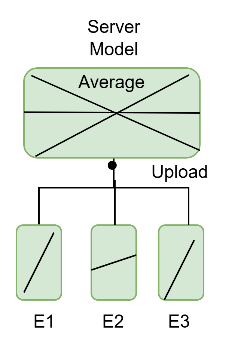
\includegraphics[height=2.7cm,keepaspectratio]{figures/fl_step_4.png} \\
\hline
5 & This trained model is sent to all participating devices and servers. & 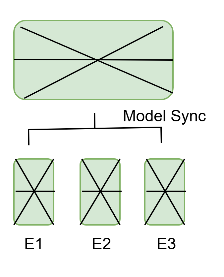
\includegraphics[height=2.7cm,keepaspectratio]{figures/fl_step_5.png} \\
\hline
\end{longtable}
\setlength{\tabcolsep}{6pt}

\subsection{Federated Learning and Personalized Recommendation System}
The decentralized ML technique known as Federated Learning (FL) allows edge devices to collaborate with a centralized server located anywhere in the world to construct a global model. While communicating with the server, these edge devices use trained parameters or gradients to keep sensitive data private.

With the support of a global server, FL enables edge devices to develop a global model in a decentralized ML approach. While communicating with the server, these edge devices use trained parameters or gradients to keep sensitive data private. In FL, a global server and other devices called local clients work as edge devices. It enables learning at edge devices, which involves training models on data distributed across thousands of devices. At the same time, it lets you improve results in both the peripheral and the central systems.

The application domain in which FL demonstrates significant advances over traditional ML solutions is Recommendation Systems. FL-based recommendation systems can learn faster and provide better recommendations. As the data remains confined to the user's environment, this innovative method allows models to be trained on devices without compromising user privacy~\cite{ref9}.

This requirement turns into the challenge of fitting large and complex neural networks on edge devices. Different approaches like Self-Governing Neural Networks (SGNN), SGNN+, and Projected Attention Network (PRADO) have been studied, which work with limited memory and computational capacity. Among these three methods, PRADO has been found to perform better for NLP applications.

\subsubsection{Transfer Learning}
Transfer learning is crucial in ML when only limited data is available for a specific problem. Usually, huge amounts of data are available for general categories, making it one of the first methods used to address cold-start users in recommendation systems and machine learning. For example, training a model to identify a specific product and other labels on a store shelf can be challenging if there are not many training photos of the specific products available. For a general domain like image training, one has sufficient training data, e.g., the ImageNet dataset. Transfer learning employs such a dataset in order to succeed in overcoming the problem of accommodating a model with a limited dataset~\cite{ref11}.

Federated Learning (FL) is closely related to Transfer Learning (TL) in the sphere of ML. TL provides a useful mechanism for utilizing pre-trained deep learning models that researchers have trained using large computational resources and a wide range of data for more specific tasks. This approach allows researchers to take tested models and apply them to concrete issues, improving efficiency and effectiveness in various applications. Building on this concept, Federated Learning, as well as Transfer Learning, are merged together to form Federated Transfer Learning (FTL). FTL is an advanced approach that ensures that FL techniques are used in various local datasets to collaboratively learn a common portion of the model architecture. This knowledge can be applied for certain tasks in each field. To illustrate, both a sentiment analysis model and a text summarization model may use a shared sentence-encoding component, which is trained through FL, making them more efficient and allowing them to perform the same tasks progressively better. The main ideas behind gaining training efficiency and iterative refining in the FL paradigm are TL and its extension, FTL~\cite{ref12}.

\subsubsection{Personalization}
According to~\cite{ref13}, personalization is a new area of research in federated learning, whereby the model learns using local data in individual devices, which leads to personalized enhancement with privacy. The raw data remains decentralized and never leaves users' devices. Personalization in federated learning occurs through updating the model parameters stored locally on users' devices or servers. These updates are typically based on each user's interactions, behaviors, or preferences. For example, in a federated learning system for a mobile keyboard app, the model may learn from each user's typing habits, frequently used words, or language preferences without sharing keystrokes or text input~\cite{ref13}.

\subsection{Categorization of Recommender Systems in FL Environment}
Federated recommendations are classified according to the recommendation system's data structure, which primarily involves two entities: users and items. Shared users or items arise from a natural connection between the parties in a Federated Recommendation. Two major types of these systems are: architecture-based and those organized by user and item features, known as Horizontal, Vertical, and Transfer federated recommendation systems~\cite{ref12}.

\subsubsection{Architecture-based}
The architecture employed for federated learning determines the form that recommendation systems can take: centralized, hierarchical, regional, or decentralized. In a federated recommendation system, all edge nodes connect to a central aggregation node, allowing local weights to be updated and models to be distributed. This setup is shown in Figure~\ref{fig:arch}. By installing numerous coordinators or regional aggregation nodes, data exchange can be reduced, and control over local devices can be increased. A more streamlined technique would be to move the aggregating function to the edge. When a global or regional server experiences heavy traffic and becomes a bottleneck, this setup serves as a viable backup plan~\cite{ref12}.

\begin{figure}[H]
\centering
\begin{minipage}[c]{0.45\textwidth}
  \centering
  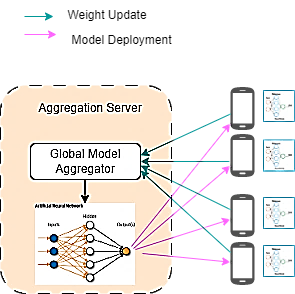
\includegraphics[width=\linewidth]{figures/image9}
  \smallskip\\
  {\small (a) Centralized}
\end{minipage}
\par\medskip
\begin{minipage}[c]{0.40\textwidth}
  \centering
  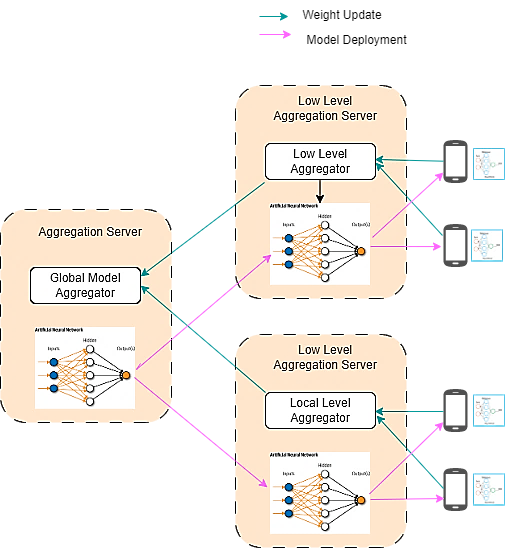
\includegraphics[width=\linewidth]{figures/image10}
  \smallskip\\
  {\small (b) Hierarchical}
\end{minipage}\hfill
\begin{minipage}[c]{0.50\textwidth}
  \centering
  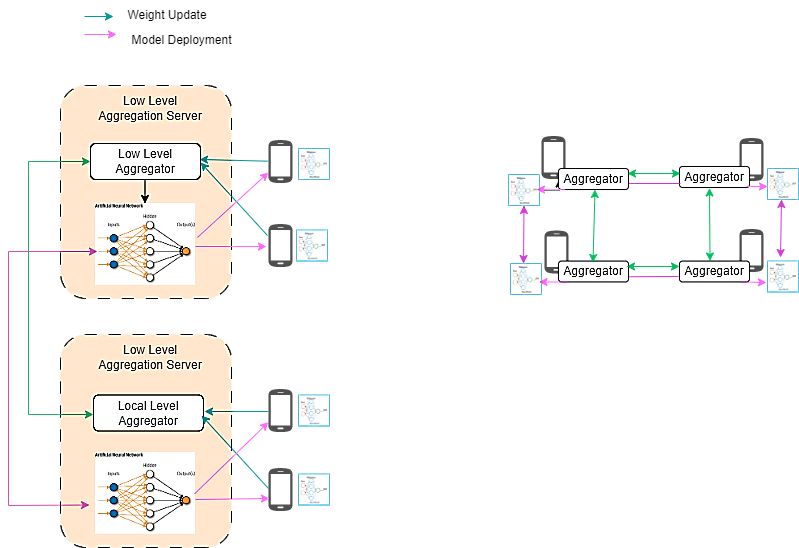
\includegraphics[width=\linewidth]{figures/image11}
  \smallskip\\
  {\small (c) Regional \hspace{1.2em} (d) Decentralized}
\end{minipage}
\caption{Communication architecture for federated recommendation: (a) Centralized, (b) Hierarchical, (c) Regional, (d) Decentralized}
\label{fig:arch}
\end{figure}

\subsubsection{Based on the distribution of Users and Item Features}
\noindent\textbf{Horizontal FedRec:} In horizontal FedRec, items are shared between parties, but not users. The parties can be individual users or groups of users. Several recent studies focus on such scenarios. Matrix factorization served as the basis for a collaborative filtering technique (FCF) proposed in~\cite{ref10}. In conventional recommendation systems, matrix factorization methods decompose the ``user-item'' rating matrix into a product of user and the item latent factor matrix. This method stores user-specific latent features locally on each device, while FCF's collective item latent features are managed by a global server. The server allots item latent factors to all devices involved in the training process at each iteration. After that, they use rating data to fine-tune their users' latent characteristics, then update the server to aggregate everything.

During the training process, no personal user data is gathered; only model updates are communicated. There is no longer any requirement for a central server thanks to the introduction of a completely distributed matrix factorization algorithm in~\cite{ref14}. Direct communication between the parties enhances the model. Furthermore, an alternate decentralized method for matrix factorization was suggested in~\cite{ref15}, in which community members, rather than outside parties, contribute local models. The algorithm's performance is considerably improved by this way.

\noindent\textbf{Vertical FedRec:} In this scenario, two entities share the same group of clients but possess different sets of items or feature spaces. These entities could be different data providers or recommenders. Many researches have been conducted to tackle the challenge of distributed learning when parties possess different features. An asynchronous stochastic gradient descent algorithm was proposed in~\cite{ref16}. To make a local prediction based on its own characteristics, either side can use any model it chooses.

Each side's training can go at their own pace within a given time frame. Reduced privacy issues are a result of this method's omission of raw data and local models. Seamlessly incorporating differential privacy greatly enhances privacy. Groups participating in vertical FedRec can have two recommenders who use different item sets. A book recommendation system and a movie recommendation system, for instance, both serve a large user base but provide distinct content. The goal is to improve recommendation algorithms using secure, privacy-preserving methods. A protected, item-based collaborative filtering method was proposed in~\cite{ref17}.

This approach enhances the effectiveness of multiple recommendation systems, each of which shows different item subsets to the same core group of users. Predicted ratings and item rankings can be calculated while maintaining both privacy and prediction accuracy.

\noindent\textbf{Transfer FedRec:} A transfer federated recommender system is characterized by the absence of shared users or items among participating parties. Typically, the involved entities are different recommender systems. A common example in Transfer FedRec is when a well-known book recommendation system collaborates with a newly launched movie recommendation system to jointly build a movie recommender system. Within this scenario, the users and items from each party are distinct. Building a federated recommender system from scratch is challenging due to the diverse range of users and items used by different organizations. To overcome these limitations, federated transfer learning~\cite{ref18} provides a useful alternative.

A few shared co-occurrence samples act as intermediaries for transferring information between domains. First, each side trains its neural network models using local data. They then work jointly to minimize the loss associated with the co-occurrence samples. Developing a secure and effective client algorithm depends on the secret sharing approach. Another scenario where this method can be useful is when items or users co-occur in the transfer FedRec setting.

\section{Research Gap}
After reviewing the literature, several gaps were identified, which motivated this research work.

\begin{enumerate}
\item The use of federated learning for cross-domain recommendation does not have a real-time implementation. How can we create and develop a federated learning framework?

\item Model training occurs on the edge device in FL, but these devices are resource-constrained, meaning they have limited computational power, memory, and more. How can these constraints be addressed?

\item How can the reviewed information be used to guide the selection of an appropriate case study for evaluating the proposed model?

\item Is the Projected Attention network suitable for improving the performance of edge devices in a Federated Learning environment?

\item Does the above technique help the model learn across domains more efficiently?
\end{enumerate}

\section{Problem Definition}
Consider a scenario where a centralized server and $M$ local clients are involved in the training process. The clients signify individual users, denoted by the set $U = \{u_1, u_2, \ldots, u_m\}$. For each user $u_i$, an emotion embedding vector $e \in \mathbb{R}^{d}$ is extracted from their reviews, forming the set of user emotions $E = \{e_1, e_2, \ldots, e_m\}$. Let $T = \{t_1, t_2, \ldots, t_n\}$ be the set of target domains, and let $V = \{v_1, v_2, \ldots, v_n\}$ denote the corresponding set of review texts associated with each item. The primary goal is to predict the appropriate emotion vector $e_i$ for each user and recommend the most relevant target item $t_j \in T$ whose reviews semantically match the user's emotional profile.

\section{Objectives of the Proposed Research}
The objective of the research is ``Designing a real-time modular federated learning system for cross-domain recommendation''.

\begin{enumerate}
\item Design and develop a scalable and modular federated framework.
\item Integrate a Projected Attention Network into a Federated Learning framework to predict emotions.
\item Develop a new federated Cross Domain Recommendation (CDR) system that uses federated transfer learning.
\item To assess the outcome of a federated CDR in comparison to baseline models.
\end{enumerate}

\section{Contribution of the Thesis}
The important contributions of the research work are:

\begin{enumerate}
\item The first contribution is the development of a federated learning framework designed to protect user data privacy. The developed framework is integrated with the Projected Attention Network to predict emotions. This process includes three modules: a projection layer to extract important features from the review text, an attention layer to capture these features, and a convolutional layer with SoftMax for classification.

\item Federated cross-domain recommendation is the second contribution, in which emotions serve as the source domain and Book, Movies, Music, and Game as the target domain. This employs a transfer learning technique in a federated environment. These techniques include aggregating weights for emotion prediction across different clients using a weighted FedAvg algorithm on the central server and an enhanced random forest classifier.

\item The modular FedCDR approach is proposed and compared in two segments: first, the model is evaluated for emotion prediction with baseline models, namely LSTM, Bi-LSTM, BERT, and PRADO; and second, it is evaluated across domains with the help of EMCDR, CDFLM, and ANR. As the third contribution, it is also compared with SOTA models like FL-EMCDR, FL-CDFLM, FL-ANR, and MFPCDR.
\end{enumerate}

\section{Organization of Thesis}
Chapter~1 introduced recommendation systems and emphasized the significance of federated learning for personalized recommendations. It also explained how federated recommendation systems are classified.

Chapter~2 reviews different studies on recommendation techniques and federated recommendation systems. It also covers the federated cross-domain recommendation system and describes the research objectives.

Chapter~3 expands the concept of emotion-driven sentiment analysis with a federated learning framework, which is part of the further research work to demonstrate cross-domain recommendations based on user emotion.

Chapter~4 details the new multi-objective Federated cross-domain recommendation that uses a PRADO.

Chapter~5 presents the findings of the proposed model and compares them with state-of-the-art systems.

Chapter~6 offers concluding remarks on the research conducted and deliberates future scope.
